\documentclass{article}
\usepackage{fbox} 
\usepackage{amsmath}
\usepackage{amssymb}
\usepackage{mathpazo}
\usepackage{pgfplots}
%\newcommand{\num}{pi}
%\pgfplotsset{compat=1.17}
 % define the plot style and the axis style
\tikzset{elegant/.style={smooth,thick,samples=50,black}}

\title{Zusammenfassung der Wissenstruktur Analysis}
\author{Bodun Du}
\begin{document}
    \maketitle
    \pagebreak
    \tableofcontents
    \pagebreak

    \section{Logik}

    \subsection{Logik der einzelnen Erscheinung}
    \begin{tabular}{ll}
        $:$ &Geltung\\
        $\exists$ &Existenz\\
        $\exists_1$ &einzigartige Existenz\\
        $\lnot $ &Verneinung\\
        $\wedge $ &gleichzeitige Existenz\\
        $\vee $ &mindestens eine Existenz\\
    \end{tabular}\\\\
    \textbf{Darstellung der Exiatenzeigenschaft:} $$Element\{Eigenschaft1; Eigenschaft2\dots\}$$
    \subsection{Menge}
    \begin{tabular}{ll}
        $\in $ &Implikation\\
        $\subset$ &Implikation aller zugehörigen Elementen\\
        $\subsetneq$ &Implikation aller zugehörigen Elementen aber Ungleichheit\\
        $\forall $ &Alle Existenzen (mit Eigenschaft\dots)\\
        $\varnothing $ &die virtuelle Menge, die von jeder Menge impliziert ist
    \end{tabular}\\\\
    \textbf{Darstellung einer Menge mit deren Elementenamen:} $$Menge=\{Elememt1, Element2\dots\}$$
    \textbf{Darstellung einer Menge mit deren Eigenschaft der Elementen:} $$Menge=\{Bedingung1; Bedingung2\dots\}$$
    \subsubsection{Erweiterung der Menge auf Logik}
    \begin{tabular}{ll}
        $\rightarrow$ &Implikation(logische Inhalte als Menge, die Untermengen impliziert)\\
        $\leftrightarrow$ &Äquivalenz(alle logische Inhalte implizieren gegenseitig)\\
        $\Rightarrow $ &Implikation mit wahrer Obermenge\\
        $\Leftrightarrow$ &wahre Äquivalenz\\
    \end{tabular}
    
    \subsubsection{die für Mengebeziehung zusammengefasste Logikbezeichungen}
    \begin{tabular}{ll}
        $\cap$ &neue Gruppe, die aus alle Elemente zweier Mengen besteht.\\&($C=A\cap B\leftrightarrow C=\{e:e\in A\wedge e\in B\} $)\\
        $\cup$ &neue Gruppe, die Elemente, die sich wowohl in A als auch in B befinden, besteht.\\&($C=A\cup B\leftrightarrow C=\{e:e\in A\vee e\in B\} $)\\
        $\backslash$ &neue Menge, die aus alle Elemente von A außer die Elemente, die auch in B befindlich\\& sind, besteht.\\&($C=A\backslash B\leftrightarrow C=\{e:e\in A\vee e\in \lnot B\} $)\\
        $\bigtriangleup $ &neue Menge, die aus alle ungleiche Elemente von A und B besteht.\\&($C=A\bigtriangleup B\leftrightarrow C=(A\backslash B)\cap (B\backslash A)  $)\\
    \end{tabular}
    
    \section{Mathematischer Beweis}
    Ein mathematischer Beweis ist die Korollar aus den Axiomen.
    \subsection{Axiom}
    Induktionsende, die stehts als wahr gegolten sind und lassen sich nicht weiter zu beweisen.\\
    \textbf{Peano-Axiome - Definition der Arithmetik}
    \footnote{Da ist die von Peano modifizierte Version, in der 0 die Kleinste Zahl von $\mathbb{N}$ ist.}
    \begin{enumerate}
        \item $0\in \mathbb{N}$\footnote{Festlegung einfachster Ursprung für weiteren Axiomen}
        \item $\forall n \in \mathbb{N} \Rightarrow \exists n' \in \mathbb{N}$\footnote{Definition der natürlichen Zahlen durch arithmischen Sinne}
        \item $\forall n \in \mathbb{N} \Rightarrow n' \neq 0 $\footnote{Vermeidung der Schleife}
        \item $\forall n,m \in \mathbb{N} :n'=m'\Rightarrow n=m$\footnote{Difinition der Wertgleichheit}
        \item $\forall X=\{0; n\in \mathbb{N}; n'\} \Rightarrow \mathbb{N} \subset X$ \footnote{Ermöglichen des Induktionsschritts}
    \end{enumerate}
    \begin{quotation}
        Man erreicht durch Zählen, ausgehend von der 1, alle natürlichen Zahlen.
        (A.Lambert, 2001-2-9)
    \end{quotation}
    \subsection{Beweisdurchfühung}
    \textbf{mathematische Induktion einer Rechenregel}
    \begin{enumerate}
        \item Induktionsanfang: Wahrnehmung der Rechenserscheinung mit einer natürlichen Zahl n (da wird oft 1 genommen)
        \item Induktionsschritt: Formulierung der Annahme durch einen Term
        \item Beweis der Induktionsannahme für n+1
        \item Erfindung der Regel für alle $n\in \mathbb{N}$
    \end{enumerate}
    \textbf{Widerspruchsentscheidung}
    \begin{enumerate}
        \item Formulierung zwei Hypothesen, die sich hinsichtlich eines Axioms zwangsläufig in der "entweder-oder-Beziehung" befinden
        \item Belegen der Widerspruchsbeobachtung einer Hypothese
    \end{enumerate}
    \pagebreak
    
    \section{Das Deduktionssystem auf Peano-Axiomen}
    \subsection{Rechenoperation}
    \begin{tabular}{ll}
        $n+m$&m-mal Wiederholung von $n'$\\
        $\sum_{n}^{m} n$& m-mal Wiederholung von $n'$ und Verbindung aller Zwischenergebnissen durch +\\
        $n\cdot m$ &m-mal Wiederholung von $a+a$   \\
        $\prod _{n}^{m} n$ & m-mal Wiederholung von $n'$ und Verbindung aller Zwischenergebissen durch $\centerdot$\\
        $n!$ & $\prod _{n=1}^{m} n$\\
        $n^m$ &m-mal Wiederholung von $n\cdot n$\\
    \end{tabular}\\\\
    Mit Wertgleichheit lässt man sich mit obrigen Rechenoperation Gleichung erstellen, sodass eine unbekannte Zahl im Term durch einer gütigen Lösung zurückzufinden ist.
    So lässt sich einige weitere Rechenoperationen durch Rückkehrung der obrigen Rechenoperationen definieren:\\
    \begin{tabular}{ll}
        - & $n+m=p\rightarrow p-m=n$ \\
        / & $n\cdot m=p \rightarrow p/m=n$\\
        $\sqrt{}$ & $n^m=q\rightarrow \sqrt[m]{q}=n $\\
        $\log$ & $n^m=q \rightarrow \log_{n}q=m$\\
    \end{tabular}
    \subsubsection*{Weiteres:}
    \begin{tabular}{ll}
        Binomialkoeffizient&  $( _{n}^{m}) = \frac{m!}{(m-n)!\cdot n!}$\\
        
    \end{tabular}\\\\
    \subsubsection{Beispiele der bewiesene Rechenregel unter den obrigen Rechenoperationen}
    \begin{tabular}{lll}
        & $a-b=a+(-b)$\\
        Kommutativgesetz& $a+b=b+a;a\cdot  b=b\cdot a$&usw.\\
        Distributivgesetz& $a\cdot b + a\cdot c= a(b+c)$&usw.\\
        Binomische Formeln& $(a+b)^2=a^2+b^2+2\cdot a\cdot b$;\\&$(a-b)^2=a^2+b^2-2\cdot a\cdot b$;\\&$(a+b)(a-b)=a^2-b^2$\\
        Unendliche Dezimalzahl& $0,\dot{9}=1\Rightarrow $\\&jede unendliche wiederholende Dezimalzahl ist ein Bruch
    \end{tabular}

    \subsection{Erweiterung der Zahlenmenge}
    Es entsteht bei der Lösung der Rückkehr-Rechenoperationen Zahlen, die teilweise nicht von $\mathbb{N}$ definiert sind, wenn in $\mathbb{N}$ statt "legale Lösungen", die mit $n';n\in \mathbb{N}$ direkt herzuleiten sind, einsetzt.\\
    So lässt sich weitere Zahlenmenge Definieren:\\
    \begin{tabular}{ll}
        $\mathbb{Z}$& alle mögliche Lösungen bei $n-m;n,m\in \mathbb{N}$\\
        $\mathbb{Q}$& alle mögliche Lösungen bei $n/m;n,m\in \mathbb{N}$\\
        $\mathbb{R}$& alle mögliche Lösungen bei $\sqrt[n]{m};n,m\in \mathbb{N}$\\
        $\mathbb{C}$& alle mögliche Lösungen bei der Kubischen Gleichung mit Bekannten$\in \mathbb{R}$\\
    \end{tabular}\\\\
    Es gilt: $\mathbb{N}\subset\mathbb{Z}\subset\mathbb{Q}\subset\mathbb{R}\subset\mathbb{C} $
    \subsection{Zahlenfolge}
    Die Zahlenmenge, deren Elemente aus einzelne Schrittergebnis einer iterativen Rechenoperation besteht.
    \pagebreak

    \section{Einfühung des Euklidischen Raums und katetischen Systems}
    \subsection{Hilberts Axiomensystem der euklidischen Geometrie}
    \begin{itemize}
        \item Axiome der Inzidenz
        \item Axiome der Anordnung
        \item Axiome der Kongruenz
        \item Axiom der Parallelen
        \item Axiom der Stetigkeit
    \end{itemize}
    \subsection{Räumliche Vorstellung der Zahlenmengen}
    \begin{itemize}
        \item $\mathbb{R}\leftrightarrow$ alle mögliche Länge einer 1-dimensionalen Gerade(Zahlengerade)
        \item $\mathbb{C}\leftrightarrow$ 3-dimensionale Erweiterung der Zahlengerade
    \end{itemize}
    \subsubsection[]{Beispiele der bewiesenen Regel unter den "Axiomen"\footnote{Der euklidische Raum ist eine logische Untermenge des Physikalischen Raums, so lässt sich das Axiomsystem weiter induzieren. Deswegen sind dessen Axiome nicht lauter.}im euklidischen Raum}
    \begin{tabular}{ll}
        Katetisches Koordinatensystem& Konstruiert man ein Bezugsgeradesystem aus zueinander\\& senkrechten Zahlengeraden(Achsen), so kann das alle im Raum\\& befindliche Orte  durch Skarlakombination Repräsentieren.\\
        $\pi=3.141\dots$ &Beziehung des Kreisumfangs und Kreisradius\\
        Satz des Phytagoras& Bezihung der Drei Kanten eines Dreiecks\\
    \end{tabular}
    \subsection{Dimension}
    je höher die Anzahl der Achsen eines kartetischen Koordinatensystems braucht, um jeden Ort eines Raum zu beschreiben, desto höher ist die Dimension dieses Raums.
    \subsection{Gleichung, Funktionsgraph}
    
    \fbox[brt]{
    \parbox{\textwidth}{
        \textbf{Gleichung}: Wertgleichheitsausdruck\\\\
        \textbf{Gleichungssystem}: Mehrere Wertgleichheitsausdrücke die (z.B. durch gemeinsame Variablen) inhaltlich zusammenhängen.
     }}
     \\\\\\
    \textbf{Funktion}: eine Gleichungsform, die die Relation mehrerer variierten Zahlen dieser Gleichung im Bezug einer vaiierten Zahl, der $f(x)$, durch einen Funktionsterm darstellt.\\
    $$f _{(x,z\dots)}=\dots$$
    \subsubsection{Funktionsgraph}
    Mittels Koordinatensystems lässt sich eine Relation der Vaiablen einer Funktion als einzelne Koordinaten eines Punkts darstellen.\\
    Soll mehrere solche Punkte vorhanden sein, lässt sich die Lösungsmenge einer Funktion versualisieren.
    \subsubsection*{Lineare Funktion}
    Bildet die Lösungsmenge ein kontinuelisches Muster, so heißt diese Funktion eine lineare Funktion und alle dazu äquivalente Gleichung lineare Gleichung.\\
    $f(x)$ entsprichen Schnittpunkt mehrerer kontinuerlichen Termen (Lösungsvektor), die eventuell auf unterschiedlichen Dimensionen sind, und hat deswegen allgemein die Form:
    $$f_{(x)}=\sum_{k=0}^{n}a_kx^k$$
    
    \fbox[blt]{
    \parbox{\textwidth}{
    \textbf{Lineare Kombination}: jeder Vektor kann umgekehrt durch seine äquivalente Lineare Funktionsterme beschrieben werden.\\\\
    \textbf{Lineare Kombinationsregel}:
     }
    } 
    \subsubsection*{"Lineare Algebra"}
    separate, abstrakte Betrachtung der Lösungsmenge der 
    \subsubsection*{Vektor}
    Abstraktion der Einzelne Punkte einer lineraren Gleichung als berechenbare Zahlenpaaren.
    \subsubsection*{Matritze}
    Erweiterung des Vektors auf dem linearen Gleichungssystem.
    \subsubsection{Beispiele der Funktion mit Funktionsgraph}
        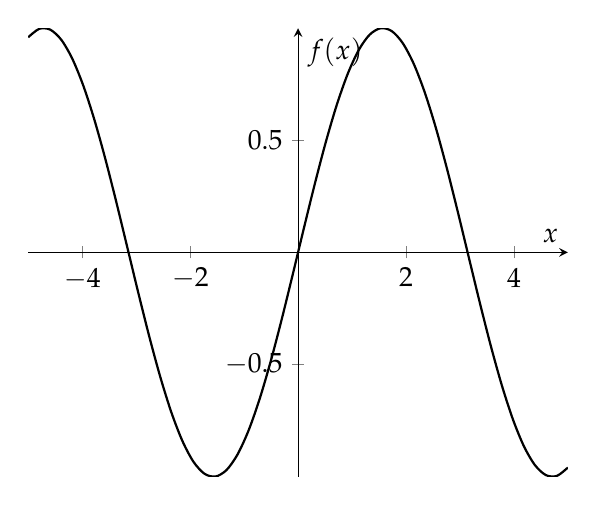
\begin{tikzpicture}% coordinates%\begin{}[]%\addplot coordinates {};%\end{}%\end{}
            \begin{axis}
                [axis x line=middle,
                 axis y line=middle,
                 ylabel=$f(x)$,
                 xlabel=$x$]
            
                \addplot[elegant] {sin(deg(x))};
            \end{axis}
        \end{tikzpicture}
    
\end{document}